\documentclass[tikz,border=2pt]{standalone}
\usetikzlibrary{positioning}
\usetikzlibrary{backgrounds}
\usetikzlibrary{fit}
\usetikzlibrary{decorations.pathreplacing}
\usetikzlibrary{arrows.meta}
\usetikzlibrary{calc}
\usepackage{amsmath}
\usepackage{amssymb}
\usepackage{graphicx}
\usepackage{tikz}
\newcommand{\preserveresulttype}[1]{
  \AtBeginEnvironment{#1}{\crefalias{theorem}{#1}}}
\newcommand{\F}{\mathbb F_2}
\newcommand{\N}{\mathbb N}
\newcommand{\Z}{\mathbb Z}
\newcommand{\cB}{\mathcal B}
\newcommand{\cR}{\mathcal R}
\newcommand{\cZ}{\mathcal Z}
\newcommand{\cH}{\mathcal H}
\newcommand{\cM}{\mathcal M}
\newcommand{\eps}{\varepsilon}
\newcommand{\EXPTIME}{\mathsf{EXPTIME}}
\newcommand{\WL}{\textnormal{\textsc{WL-Equiv}}}
\newcommand{\SubWL}{\textnormal{\textsc{Subcubic-WL-Equiv}}}
\newcommand{\id}{\operatorname{id}}
\begin{document}
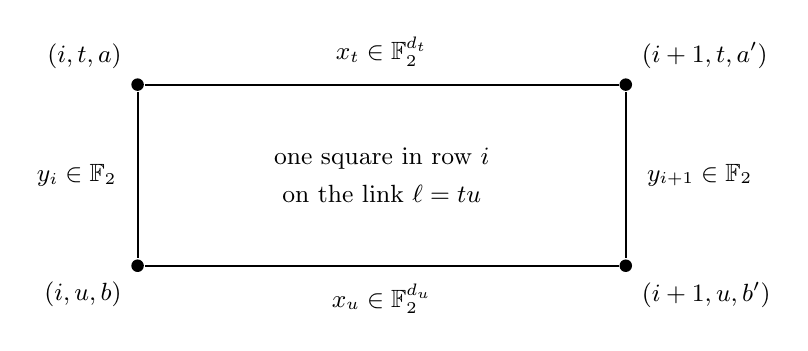
\begin{tikzpicture}[x=1cm,y=1cm,line width=.7pt,font=\small]
 \node[circle,fill,inner sep=1.6pt] (tl) at (0,0) {};
 \node[circle,fill,inner sep=1.6pt] (tr) at (6.2,0) {};
 \node[circle,fill,inner sep=1.6pt] (bl) at (0,-2.3) {};
 \node[circle,fill,inner sep=1.6pt] (br) at (6.2,-2.3) {};
 \draw (tl) -- node[above=3pt] {\(x_t\in\F^{d_t}\)} (tr);
 \draw (bl) -- node[below=3pt] {\(x_u\in\F^{d_u}\)} (br);
 \draw (tl) -- node[left=4pt] {\(y_i\in\F\)} (bl);
 \draw (tr) -- node[right=4pt] {\(y_{i+1}\in\F\)} (br);
 \node[above left=3pt] at (tl) {\((i,t,a)\)};
 \node[above right=3pt] at (tr) {\((i+1,t,a')\)};
 \node[below left=3pt] at (bl) {\((i,u,b)\)};
 \node[below right=3pt] at (br) {\((i+1,u,b')\)};
 \node[align=center] at (3.1,-1.15)
   {one square in row \(i\)\\[3pt]on the link \(\ell=tu\)};
\end{tikzpicture}
\end{document}
